\documentclass[tikz]{standalone}
\usepackage{tikz}

\begin{document}
    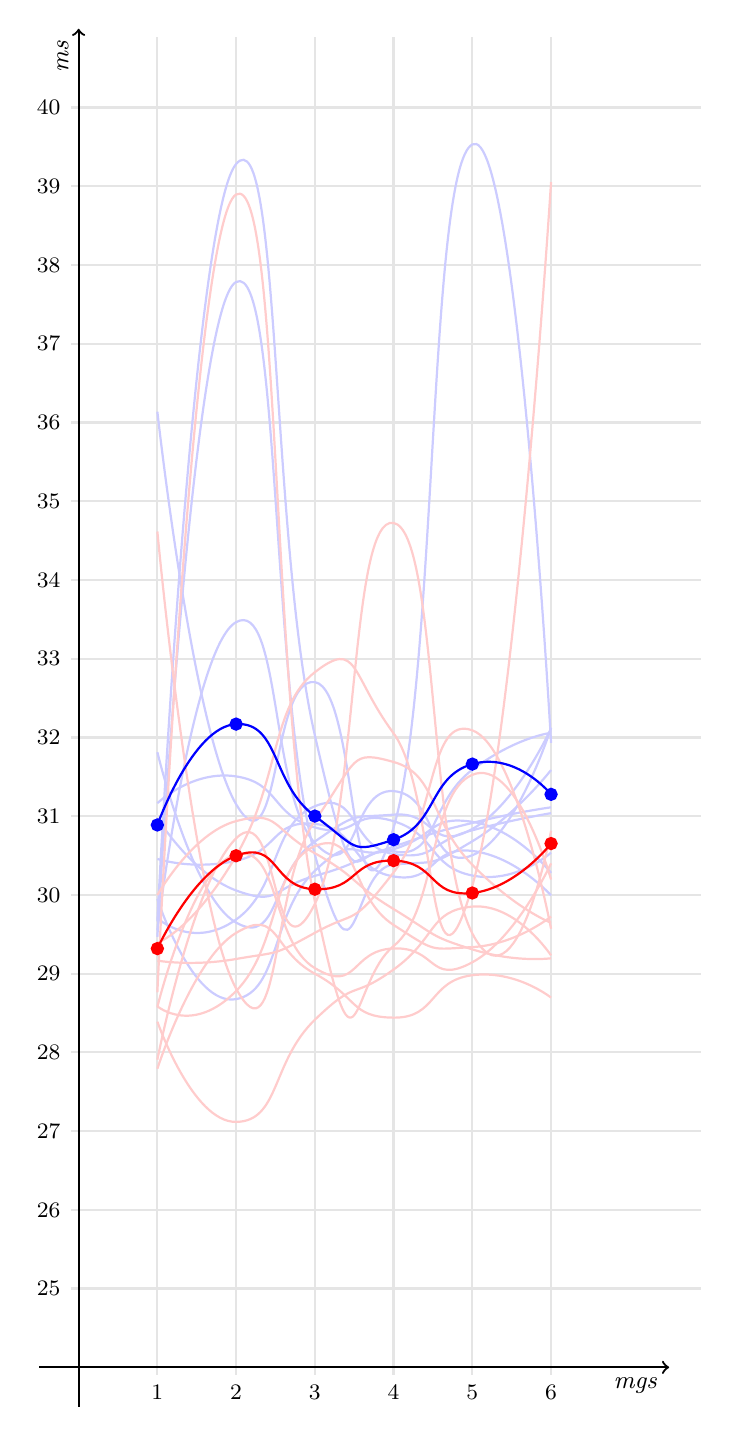
\begin{tikzpicture}[thick]

        \foreach \y in {25, 26, ..., 40} {
            \draw[gray!20] (-0.1, \y) node[left, black] {\footnotesize \y} -- ++ (8, 0);
        }
        
        
        \foreach \x in {1, 2, ..., 6}{
            \draw[gray!20] (\x, 23.9) node[below, black]{\footnotesize \x} -- ++ (0, 17);
        }

        \draw[->] (0, 23.5) -- ++ (0, 17.5) node[above left, rotate=90]{\small \textit{ms}};
        \draw[->] (-0.5, 24) -- ++ (8, 0) node[below left]{\small \textit{mgs}};


        \draw[blue!20!white] plot [smooth, tension=1] coordinates { (1, 29.662) (2, 39.282) (3, 32.027) (4, 30.555) (5, 31.589) (6, 32.058) };
        \draw[blue!20!white] plot [smooth, tension=1] coordinates { (1, 29.948) (2, 28.676) (3, 30.306) (4, 30.58) (5, 30.928) (6, 30.279) };
        \draw[blue!20!white] plot [smooth, tension=1] coordinates { (1, 29.466) (2, 37.784) (3, 30.512) (4, 30.386) (5, 30.681) (6, 31.586) };
        \draw[blue!20!white] plot [smooth, tension=1] coordinates { (1, 29.705) (2, 29.687) (3, 31.126) (4, 30.519) (5, 30.821) (6, 31.038) };
        \draw[blue!20!white] plot [smooth, tension=1] coordinates { (1, 36.137) (2, 31.152) (3, 32.702) (4, 30.854) (5, 39.531) (6, 31.931) };
        \draw[blue!20!white] plot [smooth, tension=1] coordinates { (1, 29.551) (2, 33.464) (3, 30.66) (4, 31.318) (5, 30.503) (6, 32.122) };
        \draw[blue!20!white] plot [smooth, tension=1] coordinates { (1, 30.974) (2, 30.056) (3, 30.241) (4, 30.613) (5, 30.914) (6, 31.112) };
        \draw[blue!20!white] plot [smooth, tension=1] coordinates { (1, 31.164) (2, 31.505) (3, 30.857) (4, 30.936) (5, 30.246) (6, 30.537) };
        \draw[blue!20!white] plot [smooth, tension=1] coordinates { (1, 31.812) (2, 29.648) (3, 30.678) (4, 31.019) (5, 30.837) (6, 32.115) };
        \draw[blue!20!white] plot [smooth, tension=1] coordinates { (1, 30.457) (2, 30.433) (3, 30.902) (4, 30.234) (5, 30.558) (6, 29.993) };
        
        \draw[red!20!white] plot [smooth, tension=1] coordinates { (1, 28.585) (2, 28.779) (3, 30.619) (4, 29.618) (5, 29.337) (6, 29.725) };
        \draw[red!20!white] plot [smooth, tension=1] coordinates { (1, 29.391) (2, 30.496) (3, 32.828) (4, 32.052) (5, 30.116) (6, 39.053) };
        \draw[red!20!white] plot [smooth, tension=1] coordinates { (1, 28.763) (2, 38.895) (3, 29.917) (4, 29.35) (5, 31.525) (6, 30.195) };
        \draw[red!20!white] plot [smooth, tension=1] coordinates { (1, 28.39) (2, 27.117) (3, 28.414) (4, 29.052) (5, 29.851) (6, 29.231) };
        \draw[red!20!white] plot [smooth, tension=1] coordinates { (1, 28.578) (2, 30.515) (3, 29.07) (4, 29.32) (5, 29.144) (6, 30.4) };
        \draw[red!20!white] plot [smooth, tension=1] coordinates { (1, 29.997) (2, 30.937) (3, 30.529) (4, 29.82) (5, 29.308) (6, 29.195) };
        \draw[red!20!white] plot [smooth, tension=1] coordinates { (1, 29.165) (2, 29.186) (3, 29.518) (4, 30.285) (5, 32.09) (6, 29.57) };
        \draw[red!20!white] plot [smooth, tension=1] coordinates { (1, 27.792) (2, 29.517) (3, 28.999) (4, 28.441) (5, 28.98) (6, 28.695) };
        \draw[red!20!white] plot [smooth, tension=1] coordinates { (1, 34.615) (2, 28.81) (3, 30.94) (4, 31.688) (5, 30.382) (6, 29.646) };
        \draw[red!20!white] plot [smooth, tension=1] coordinates { (1, 27.907) (2, 30.718) (3, 29.886) (4, 34.724) (5, 29.51) (6, 30.814) };
        
        \draw[blue] plot [smooth, tension=1, mark=*] coordinates { (1, 30.888) (2, 32.169) (3, 31.001) (4, 30.701) (5, 31.661) (6, 31.277) };
        \draw[red] plot [smooth, tension=1, mark=*] coordinates { (1, 29.318) (2, 30.497) (3, 30.072) (4, 30.435) (5, 30.024) (6, 30.652) };
    \end{tikzpicture}
\end{document}